\section{Aggregates and Aggregates-NotSameBeads} \label{sec:Aggregates}

These utilities determine which molecules belong to which aggregates (note that
\enquote{aggregate} is used for any supramolecular structure) according to a
simple criterion: two molecules belong to the same aggregate if they share at
least a specified number of contact pairs. A contact pair is a pair of two beads
belonging to different molecules which are closer than a specified distance. The
information is written into an \tt{.agg} text file described in
Section~\ref{sec:AggFile}.

% The number of contact pairs, the distance, and bead type(s) to use for
% aggregate determination are all arguments of the utilities.  Any molecule
% type(s) can be excluded from aggregate determination (\tt{-x <mol
% name(s)>} option); they are also excluded from the output \tt{agg}
% file).  Moreover, any molecules close to specified molecule(s) can be
% excluded (\tt{-xm <mol name(s)>} option); here, \enquote{close} means
% any of the bead types used in aggregate determination is closer than
% \tt{<distance>} to any bead of the specified molecule.

Periodic boundary conditions can be removed from whole aggregates via the
\tt{-j} option; the aggregate's centre of mass is always inside the simulation
box. This is useful for visualization (an aggregate will no longer be split by
the walls of the simulation box, but it may stretch far outside the boundaries
of the box) as well as for further analysis (the other utilities do not have to
join the aggregates, possibly greatly speeding up subsequent analyses).

While the \tt{Aggregates} utility uses all possible pairs of given bead types,
\tt{Aggrega}-\tt{tes-NotSameBeads} does not use same-type pairs. For example, if
bead types \tt{A} and \tt{B} are given, \tt{Aggregates} will use all three
possible bead type pairs (i.e., \tt{A-A}, \tt{A-B}, and \tt{B-B}), but
\tt{Aggregates-NotSameBeads} will use only \tt{A-B} bead type pairs.
Fig~\ref{fig:AggCheck} illustrates the behaviour: using \tt{Aggregates ... A B}
would find one contact pair between molecules 1 and 2 and two contacts between
molecules 2 and 3, whereas \tt{Aggregates-NotSameBeads ... A B} would ignore A-A
and B-B pairs, finding no contact pair between molecules 1 and 2 and only one
between molecules 2 and 3.

\begin{figure}
  \centering
  \begin{minipage}{0.45\textwidth}
    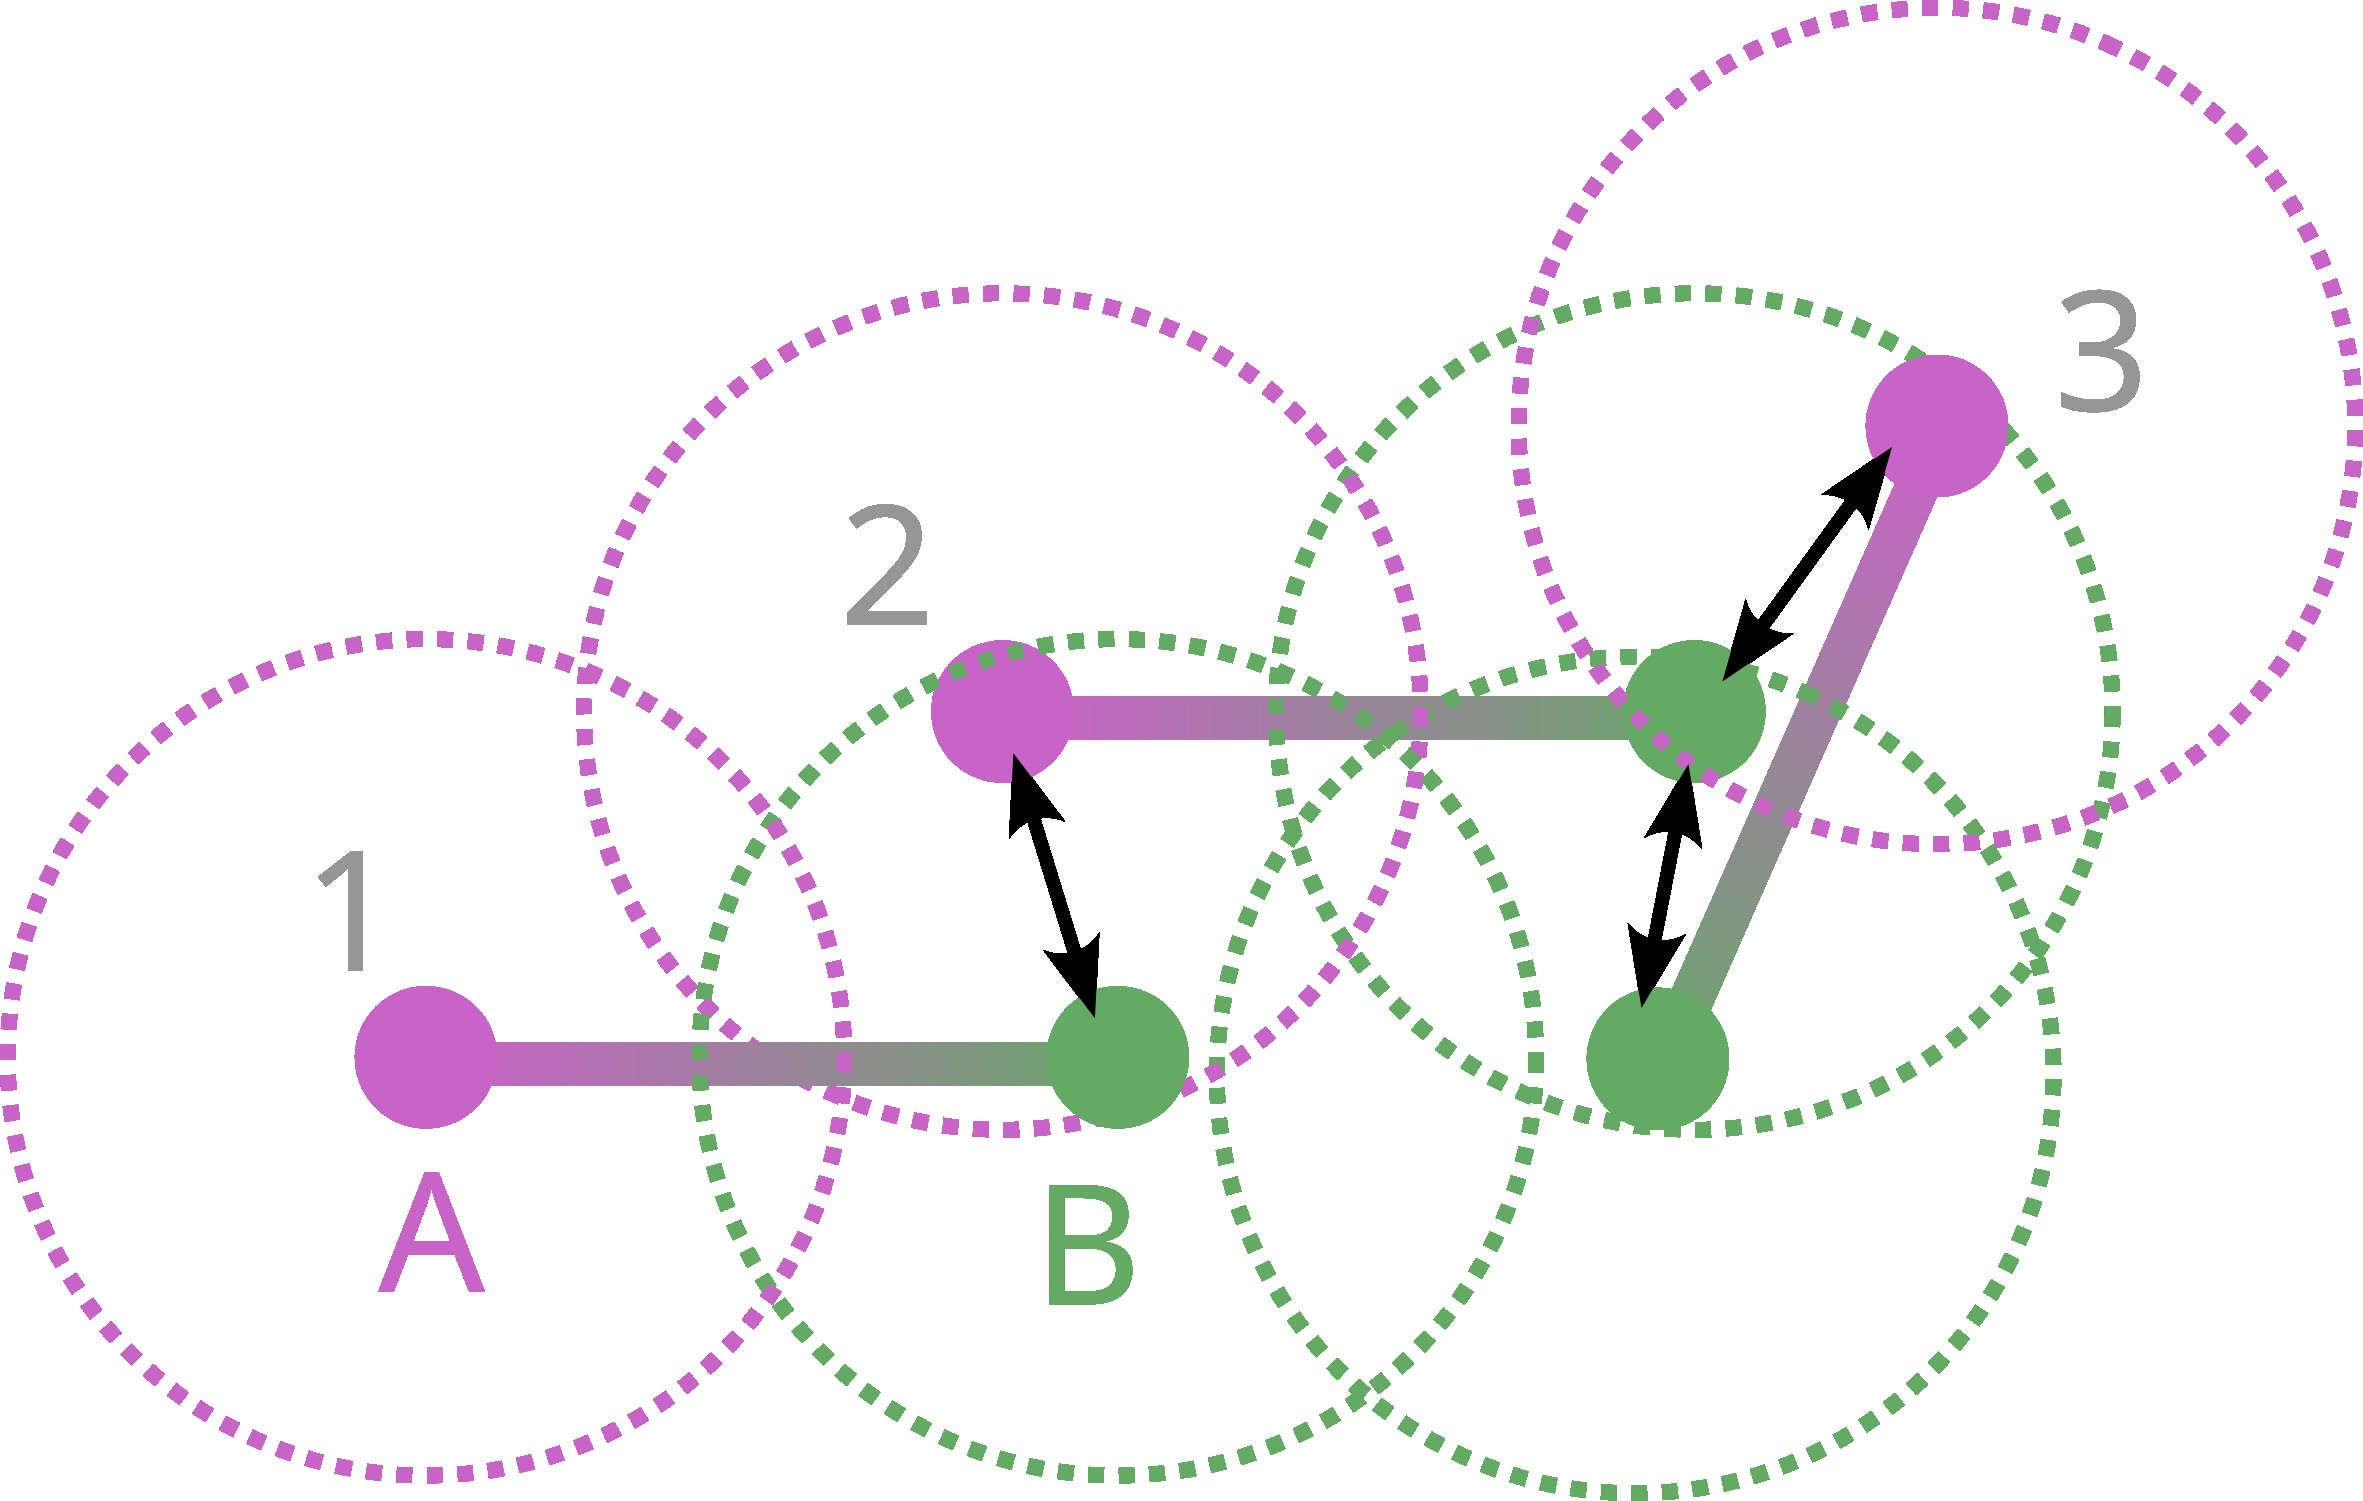
\includegraphics[scale=0.6]{AggregateCheck.jpg}
  \end{minipage}
  \begin{minipage}{0.5\textwidth}
    \tt{Aggregates ... A B}\\
    \-\hspace{30pt}$\Rightarrow$ 3 contact pairs\\
    \tt{Aggregates-NotSameBeads ... A B}\\
    \-\hspace{30pt}$\Rightarrow$ 2 contact pairs\\
  \end{minipage}
  \caption{
    Simple example of distance checks---three two-bead molecules, where dotted
    lines represent maximum pair distance (\tt{-d} option) and black arrows show
    contact pairs. Note the same bead can be a part of multiple pairs.
  }
  \label{fig:AggCheck}
\end{figure}

If \tt{-w} option is used, the utilities also take the found aggregates, testing
which are touching the specified wall(s) and saving those touching the wall(s)
and those in bulk into two extra \tt{.agg} files. The wall(s) are specified via
the \tt{<a>} argument, which defines the axis perpendicular to the wall (the
argument must be \tt{x}, \tt{y}, or \tt{z}), and numeric argument(s), which
define the coordinate(s) of the wall(s) along the axis. For example, assuming a
simulation box with size $10^3$ and a slit configuration with two walls in the
xy-plane 1 distance unit from the box edges, then \tt{-w z 1 9} would be used.
The distance for checking whether a bead touches the wall is the same as the one
for determining bead contact pairs. Aggregate data are saved into two extra
\tt{.agg} files with names based on the main output \tt{<out.agg>} -- \tt{-w}
and \tt{-no_w} is placed before the \tt{.agg} extension.

Note that when \tt{-st}, \tt{-e}, or \tt{-sk} options are used, the resulting
\tt{agg} file is no longer coupled to the original coordinate file (i.e., they
cannot be used together for further analyses), but it is coupled to the optional
output file with joined coordinates (\tt{-j} option).

\vspace{1em}
\noindent
Usage: \tt{Aggregates <input> <out.agg> <bead type(s)> [options]}
\noindent
\begin{longtable}{p{0.22\textwidth}p{0.724\textwidth}}
  \toprule
  \multicolumn{2}{l}{Mandatory arguments}\\
  \midrule
  \tt{<input>}        & input coordinate file\\
  \tt{<out.agg>}      & output \tt{agg} file\\
  \midrule
  \multicolumn{2}{l}{Options}\\
  \midrule
  \tt{-d <num>}       & maximum distance for contact (default: 1)\\
  \tt{-c <num>}       & minimum number of contacts (default: 1)\\
  \tt{-j <file>}      & save coordinates of joined aggregate to
                        a coordinate file\\
  \midrule
  \multicolumn{2}{l}{Other options (see the beginning of 
                     Chapter~\ref{chap:Utils})}\\
  \midrule
  \multicolumn{2}{l}{\tt{-st},
                     \tt{-e},
                     \tt{-sk},
                     \tt{-i},
                     \tt{--verbose},
                     \tt{--silent},
                     \tt{--help},
                     \tt{--version}}\\
  \bottomrule
\end{longtable}
